% siminos/froehlich/slice/flotsam.tex  called by FrCv11.tex
% $Author$ $Date$

\section{Flotsam}
\label{sec:flotsam}

%\ifboyscout
%\subsubsection{Subsubsection header}
%[Just checking what the header looks like]
%\else
%\fi

---
  %
  %
\PC{{\bf to Stefan}:
write abstract, intro, conclusions often!
This might be the only part of this text that most
people glance at.
%PC 2010-09-30: planted an error into the abstract, just to see how
%   often do you edit it.
%
%
   When you write a project report or a research article, you always
   write abstract, introduction and conclusions first, and then keep
   rewriting them often. They are the most important parts of the text,
   as that is for most people only parts they will look at.
   }

													\toCB

-------------

symmetry reduction = lowering the order\rf{ArKoNe88} % (Arn Kozl Neist)

-------------

{\bf PC}{still have to derive the general case: ``
Let $\sliceTan{}$ be a vector normal to the plane of the slice. Then the
dynamics within the slice are given by
\bea
\dot{\gSpace_a}(\sspRed) &=& \frac{\braket{\vel(\sspRed)}{\sliceTan{a}}}
               {\braket{\groupTan(\sspRed)}{\sliceTan{}}}
\continue
\velRed(\sspRed) &=& \vel(\sspRed)
   -\dot{\gSpace}(\sspRed) \cdot \groupTan(\sspRed)
\label{SF:sliceEas}
\eea
where $\velRed(\sspRed)$ is the velocity in the slice.
    ''}

-------------

If $\ssp(\tau)$ is a solution to the dynamical equations, then
$\LieEl\,\ssp(\tau)$ is also a solution.

Most of the Lie groups that we will only be considering here are
compact.

The $L^2$ norm of $\groupTan(u)$ is weighted by
the quadratic Casimir \refeq{QuadCasimir}. For \SOn{2} this is
$C_2^{(m)} = m^2$,
\beq
\oint \frac{d\gSpace}{2\pi}
     \, (\Lg u(\gSpace))^T \Lg u(2\pi-\gSpace)
= \sum_{m=1}^\infty m^2 \left(a_m^2 + b_m^2\right)
\,.
\ee{tangL2norm}

  %
We only care about those that are local (and preferably global) {\em
minima}, for which all the eigenvalues of the symmetric matrix
$[N\!\times\!N]$ matrix of second derivatives of distance,
\beq
\frac{\partial^2}
     {\partial \gSpace_a \partial \gSpace_b}
        |\sspRed - \slicep|^2
    =
%  - \braket{\Lg_a e^{\gSpace \cdot \Lg} \ssp}{\sliceTan{b}}=
  - \braket{\groupTan_a(\sspRed)}{\sliceTan{b}}=
  \braket{\sspRed}{\Lg_a \Lg_b\slicep}
\ee{PCinflPoint}
are positive. In practice we do not need to actually compute
this matrix, we simply pick from among the local minima
the infimum of the distance.

{\bf PC:}{ could it be that inflections are generic only for \SOn{2},
        but of higher codimension and thus not encountered
        by 1\dmn\ time trajectory for higher-dimensional Lie groups?}


-------------

{\bf PC:}{
{\bf Tessellation of the \reducedsp\ by two or many slices:
how to implement it?}
See \HREF{http://en.wikipedia.org/wiki/Voronoi_diagram}
{wiki on Voronoi diagrams}.
We have to study Roweis  and Saul\rf{RoSa00}
\emph{``Nonlinear dimensionality reduction by locally linear embedding.''}
A sobering fact: Rowais, assistant professor at N.Y.U., a young
star in the field and universally liked, jumped out of his Washington
Square apartment earlier this year.
	}


%\ES{ If find this derivation confusing and hard to follow,
%although it illustrates a very simple fact, encapsulated in this last sentence.
%Contrary to what you say here, in your derivation you start by rotating
%the template $\slicep$, but then also rotate the \statesp\ point $\ssp$ and you
%tacitly use the fact that in order to minimize distance either way you have
%to rotate by the same angle. I don't disagree, but it might be hard for the
%casual reader to follow. I propose the following simplification of the
%derivation, in the spirit of your last sentence: Look instead for minima of
%\[
%	|\LieEl(\gSpace)x-\slicep|^2\,,	
%\]
%to get
%\[
% \frac{\partial ~~}{\partial \gSpace_a}	|\LieEl(\gSpace)x-\slicep|^2 \sim
%		\braket{\Lg_{a}\sspRed}{\sspRed-\slicep}=0\,,
%\]
%and finally use antisymmetry of $\Lg_{a}$ (twice) to write this as
%$\braket{\sspRed}{\sliceTan{a}} =0$.
%
%I also suggest that it might benefit the reader to introduce the group
%angle parameterization earlier in this section, \ie\ use
%$\LieEl(\gSpace)\ssp$ instead of $\LieEl\ssp$, \etc
%}

-------------

Shift in time to the closest passage\rf{pchaot,MFKM10,CviGib10}:
`close recurrence.'

-------------

Unattended to, a symmetry can induce drifts along group orbit directions
and be a great nuisance; deftly deployed it can be a powerful tool in
simplifying physical problems.

Symmetry strongly constrains the form of solutions and their
bifurcations, if appropriately implemented, it can significantly
accelerate convergence of numerical algorithms, it splits the dynamical
\statesp\ into chains of lower-dimensional flow-invariant subspaces,
dictates its invariant partitions and the symbolic dynamics.

-------------

By construction, $S$ lies within, and is lower-dimensional than
the \reducedsp, $\sspRSing \in S \subset \pSRed$.

	{\bf PC to Stefan:} In \reffig{fig:dthetasing}\,(b) and \reffig{fig:singpass}\,(a)
you use a full \statesp\ perturbation $\delta \ssp$. Would it be more consistent
to perturb with $\delta \sspRed$?
\\
    {\bf SF:} I used the perturbation $\delta \ssp$ because I was calculating
    the trajectories in the full space and then reducing them.
    dy=(-0.0246486, 0.00417712, 0., 0., 0.) if you want to use it.
\\
{\bf PC to Stefan:}
full \statesp\ perturbation $\delta \ssp$ is good enough, we stick to it.

-------------

%% In FrCv11.tex replaced by f_1_08_1.png
%%{Hyp} %{fig6} and {tr:fig6} in ChaosBook
%% \HREF{http://chaosbook.org/overheads/trace/Tesselate.jpg}
%%%%%%%%%%%%%%%%%%%%%%%%%%%%%%%%%%%%%%%%%%%%%%%%%%%
% \begin{figure}
% \begin{center}
%%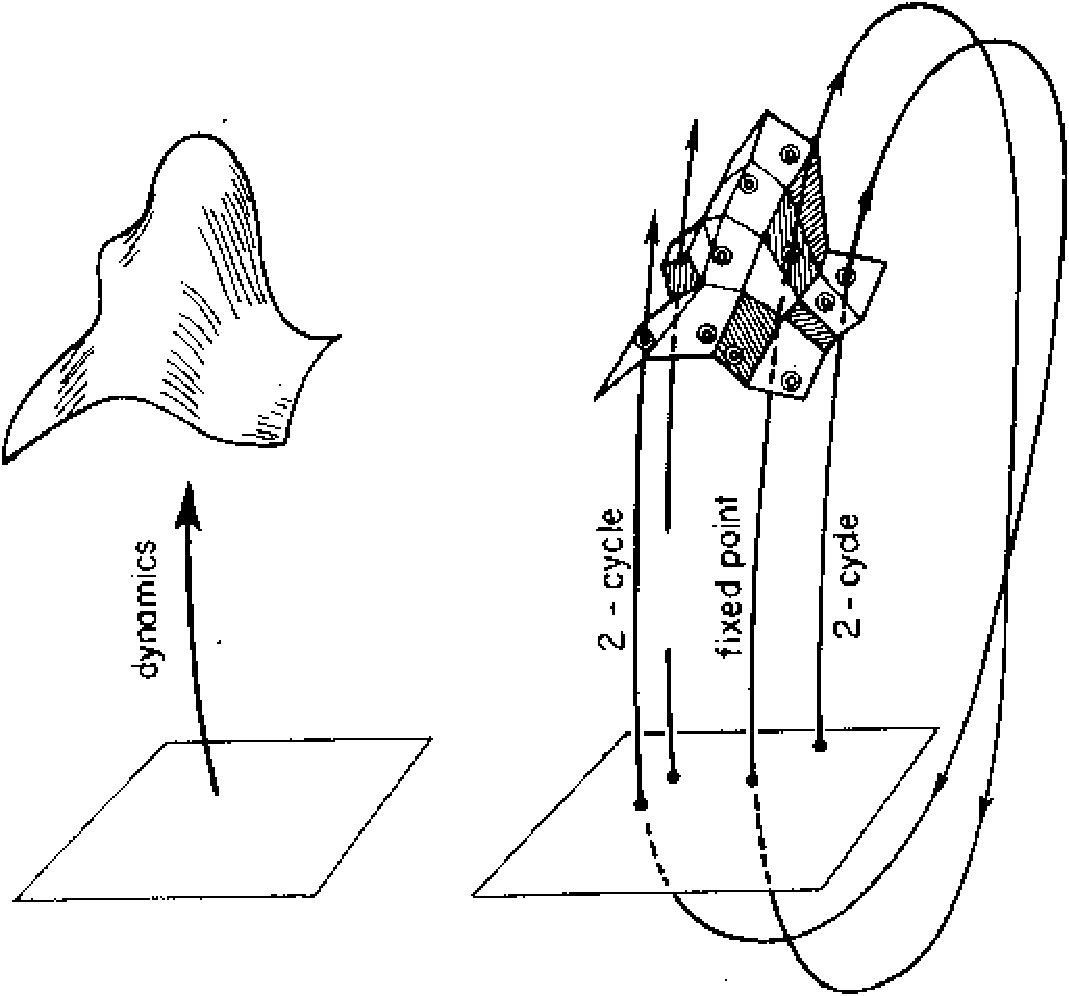
\includegraphics[width=0.35\textwidth]{f_1_08_1}
% \end{center}
% \caption{\label{fig:Tesselate}
%Smooth dynamics  (left frame) tesselated by the skeleton of periodic
%points, together with their linearized neighborhoods, (right frame).
%Indicated are segments of two 1-cycles and a 2-cycle that alternates
%between the neighborhoods of the two 1-cycles, shadowing first one, and
%then the other
%(from \wwwcb{}).
%  }\end{figure}
%%%%%%%%%%%%%%%%%%%%%%%%%%%%%%%%%%%%%%%%%%%%%%%%%%%
%%
%


 This tessellation is akin to the
%\HREF{http://en.wikipedia.org/wiki/Vector_quantization}
{`vector quantization,'} (`block quantization,'  `pattern matching quantization'),
a computer science data compression method where sets of points are
clustered by their distance to `prototype' or `reference' points. The
method encodes values from a multidimensional vector space into a
`codebook,' a finite set of values from a discrete space of a lower
dimension; \ie, what in the theory of dynamical systems is called
`symbolic dynamics.'

Ridges (intersection boundaries between different slices) are themselves
hyperplanes of lower dimensions, easy to compute once we have picked
the set of {\template s}. To find what slice a given full \statesp\
trajectory point is in, one rotates with respect to each slice, and
checks whether the given group orbit belongs to it. In the \reducedsp\
the trajectory is integrated within a given slice until it hits a ridge -
then one switches to the next slice across the boundary.

Ridges are of Lebesgue measure zero, no way you would hit them.

We do not need to be very precise about the instant
where we switch, as long as we are away from either slice's singularity
subspace.

The \reducedsp\ tessellation by a set of slices
locked relative to each other by the shortest unstable manifold segments
offers a better approximation to distances between points on an attractor
of a nonlinear flow.

That means that the neighborhood - bounded by intersections with
neighboring slices is sufficiently small that group tangent space is
nowhere within the slice - works in smooth flows for sufficiently small
neighborhoods.

-------------

{\bf PC to Stefan}:
	While `fixes' is a correctly used math word, I tend to avoid it 	
as it violates the common usage; $\Lg_1$ does not (transitively) `fix'
anything, 	it simply does not act upon $b$ coordinates.

-------------

{\bf 2011-01-15 PC}: removed Stefan's `` When the group tangent of the reduced
trajectory points in the slice, the equation for $\dot{\gSpace}$ is not
defined and the trajectory passes through a `singularity'. '' from Moving
frames section; this remark belongs to the next section.
